\documentclass[aspectratio=169,17pt,fleqn]{beamer}

\usetheme{Madrid}
\usecolortheme{dolphin}
\setbeamertemplate{navigation symbols}{}
\setbeamertemplate{footline}[frame number]

\usepackage{amsmath,amssymb,array}

\usepackage{booktabs}



\usepackage{fontspec}    
\usepackage{unicode-math}  

\AtBeginSection[]{
  \begin{frame}
    \centering
    \vfill
    \Large\insertsectionhead
    \vfill
  \end{frame}
}

\usepackage{tikz}
\usetikzlibrary{positioning,matrix,backgrounds}
\usepackage{tikz-cd}


\title{Metatheory}
\author{PHI~201 -- Introductory Logic}
\date{Week 11}

\begin{document}

\frame{\titlepage}

\begin{frame}{Remaining tasks}

  \begin{enumerate}
  \item Figure out how to prove harder things (more reliably)
    \begin{itemize}
    \item Example: $\vdash\exists x\forall y(Fx\to Fy)$
    \item Idea: Convert semantic intuition into proof
    \end{itemize}
  \item Learn how to reason \emph{about} propositional logic
    \begin{itemize}
    \item New axiom schema: mathematical induction
    \item Main results: soundness, completeness
    \end{itemize}
  \end{enumerate}

  \end{frame}

\section{A theory \emph{about} propositional logic}  

\begin{frame}

\begin{itemize}  
\item You'll keep using logic, but most of you won't study logic again
  in a formal setting like this one.
\item But learning about how logic works will help you become better
  at doing logic.
  \begin{itemize}
  \item Analogy to an athlete and understanding physiology and
    nutrition.
  \item But that analogy fails to capture the fascinating fact that
    studying logic is another use of logic.
  \end{itemize}  
\end{itemize}

\end{frame}

\begin{frame}

\begin{itemize}
\item To formalize a theory in predicate logic, one chooses some basic
  vocabulary (names, predicates, relations, functions).
\item We are going to be talking about \alert{sentences},
  \alert{sequents}, \alert{valuations}, etc. So, for example, we
  would have a predicate symbol $\mathsf{Sent}(x)$ to mean that $x$ is
  a sentence, and a relation symbol $\mathsf{Seq}(x_1,\dots ,x_n,y)$
  to mean that there is a valid proof whose last line has formula $y$
  with dependencies $x_1,\dots ,x_n$.
\end{itemize}


\end{frame}

\section{Mathematical induction}

\begin{frame}

\begin{itemize}
\item The interesting theorems about propositional logic involve
  claims about infinite sets. For example:
  \begin{quote} For every sentence $\varphi$, $\varphi$ is provably
    equivalent to a sentence in which $\wedge$ does not
    occur. \end{quote}
\item But our infinite sets are generated from a finite number of
  cases by a finite number of rules. There is a special method of
  proof for such sets: \alert{mathematical induction}.
\end{itemize}

\end{frame}

\begin{frame}{Aside: Function symbols}

  An $n$-ary function symbol $f$ combines with $n$ terms to give
  another term.

  \bigskip \begin{block}{Terms}
    \begin{itemize}
    \item Base case: Variables and names are terms.
    \item Inductive case: If $t_1,\dots ,t_n$ are terms, and $f$ is an
      $n$-ary function symbol, then $f(t_1,\dots ,t_n)$ are terms.
    \end{itemize}
  \end{block}



\end{frame}

\begin{frame}{Induction inference rule for arithmetic}

  \noindent 
    \begin{tabular}{p{7cm} l}
      $\varphi(0)$ & base case  \\[0.3em]
      $\forall x(\varphi(x) \rightarrow
                \varphi(x+1))$ & inductive step \\[1.3em]
      $\forall x\,\varphi(x)$ & conclusion 
\end{tabular}

\end{frame}

{
\setbeamertemplate{background}{
  
\begin{tikzpicture}[remember picture,overlay]
    \draw[step=0.5cm,gray!30] (current page.south west) grid (current page.north east);
  \end{tikzpicture}
}

\begin{frame}

  \textbf{Fact:} Every number is either even or odd.

  \noindent \[ \varphi (x) \:\equiv \: (\exists y(x=y+y)\vee \exists z(x=z+z+1)) \]

  \vspace{9em}


\end{frame}

}

\section{Induction on the construction of sentences}

\begin{frame}{Derivation rule for $\{ \vee ,\neg \}$ sentences}

\begin{block}{}
\begin{tabular}{@{}lp{9.5cm}r@{}}
  (1) & Atomic sentences have property $X$.                          
  & \hspace{1cm}\textit{base case} \\[0.6em]

  (2) & If $\varphi$ and $\psi$ have property $X$, then 
        $\varphi \lor \psi$ has property $X$.  
    & \hspace{1cm}\textit{induction $\lor$} \\[0.6em]

  (3) & If $\varphi$ has property $X$, then $\lnot\varphi$ 
        has property $X$.                                
  & \hspace{1cm}\textit{induction $\lnot$} \\[0.6em]
  \midrule
  (C) & Every sentence built from atomics using $\vee$ and $\neg$ has property $X$.      
  & \hspace{1cm}\textit{conclusion}
\end{tabular}
\end{block}

\end{frame}

\begin{frame}[fragile]

  \textbf{Fact:} Every sentence built from the atomic sentence $P$,
  using $\vee$ and $\neg$, is provably equivalent to one of the four
  sentences in the diamond:

  \bigskip \noindent \[ \begin{tikzcd} & \arrow[-]{dl} \top \arrow[-]{dr} & \\
    P & & \neg P \\
    & \arrow[-]{ul} \bot \arrow[-]{ur} & \end{tikzcd} \]


\end{frame}

%% give argument 

\begin{frame}

  \textbf{Fact:} Every sentence built from $P$, using all
  propositional connectives, is provably equivalent to a sentence that
  only contains $\vee$ and $\neg$.

  \vspace{10em}

\end{frame}

\section{Truth functions}

\begin{frame}
  \frametitle{Unary truth-functions}

  A unary truth-function is a map from $\{0,1\}$ to $\{0,1\}$. There
  are exactly \textbf{4} possibilities:

  \begin{itemize}
    \item identity: $0\mapsto 0,\; 1\mapsto 1$
    \item flip: $0\mapsto 1,\; 1\mapsto 0$
    \item constant $0$: $0,1 \mapsto 0$
    \item constant $1$: $0,1 \mapsto 1$
  \end{itemize}

  \medskip \noindent Each can be expressed with our connectives.
\end{frame}

\begin{frame}{Binary truth-functions}

  A binary truth-function is a map from $\{0,1\}\times\{ 0,1\}$ to
  $\{ 0,1\}$.

  \medskip There are $4$ elements of $\{ 0,1\}\times\{ 0,1\}$.

  \medskip Binary truth-functions correspond one-to-one to subsets of
  $\{0,1\}\times\{0,1\}$.

  \medskip There are $2^4=16$ binary truth functions.


\end{frame}

\begin{frame}

  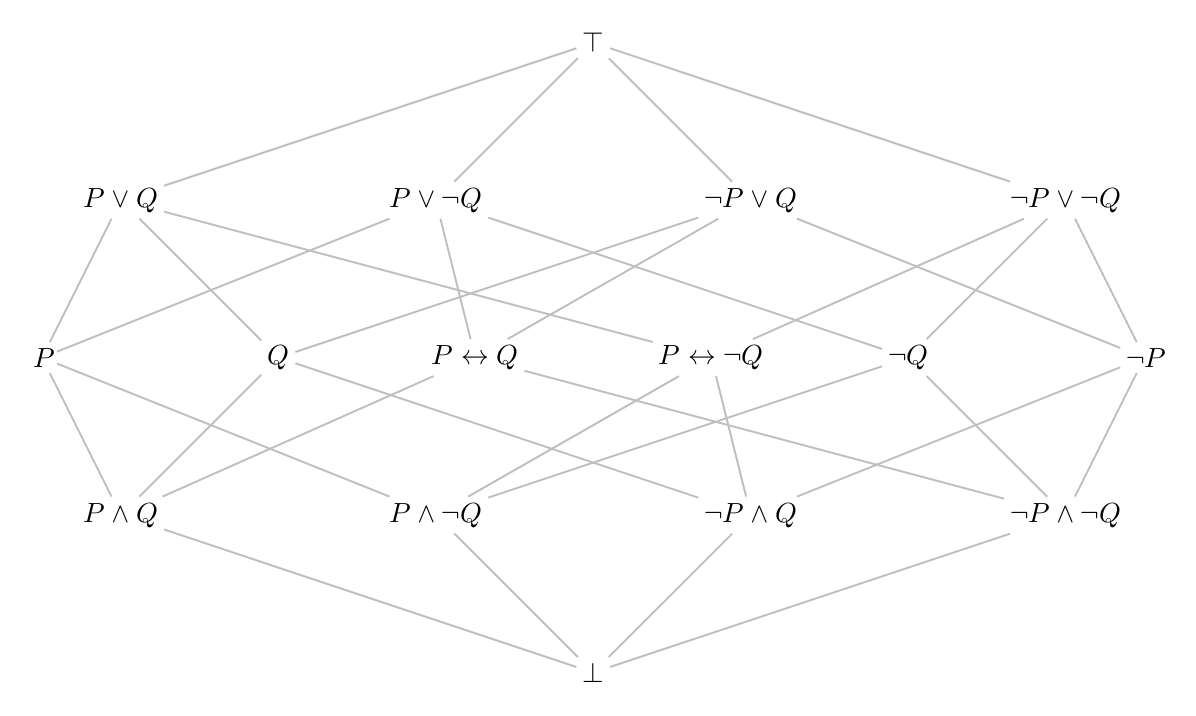
\begin{tikzpicture}[
    source/.style={inner sep=2pt},
    edge/.style={line width=0.7pt, draw=gray!50}
    ]
  % \begin{tikzpicture}[source/.style={draw,thick,rounded corners,inner sep=2pt}]
  % bottom and top
  \node[source] (min) at (0,-1) {$\bot$};
  \node[source] (max) at (0,7) {$\top$};

  % layer A (conjunctions)
  \node[source] (A1) at (-6,1) {$P\wedge Q$};
  \node[source] (A2) at (-2,1) {$P\wedge \neg Q$};
  \node[source] (A3) at ( 2,1) {$\neg P\wedge Q$};
  \node[source] (A4) at ( 6,1) {$\neg P\wedge \neg Q$};

  % layer B (atoms & biconditionals)
  \node[source] (B1) at (-7,3) {$P$};
  \node[source] (B2) at (-4,3) {$Q$};
  \node[source] (B3) at (-1.5,3) {$P\leftrightarrow Q$};
  \node[source] (B4) at (1.5,3) {$P\leftrightarrow \neg Q$};
  \node[source] (B7) at ( 4,3) {$\neg Q$};
  \node[source] (B8) at ( 7,3) {$\neg P$};

  % layer C (disjunctions)
  \node[source] (C1) at (-6,5) {$P\vee Q$};
  \node[source] (C2) at (-2,5) {$P\vee \neg Q$};
  \node[source] (C3) at ( 2,5) {$\neg P\vee Q$};
  \node[source] (C4) at ( 6,5) {$\neg P\vee \neg Q$};

  % edges from bottom
  \draw[edge] (min) -- (A1);
  \draw[edge] (min) -- (A2);
  \draw[edge] (min) -- (A3);
  \draw[edge] (min) -- (A4);

  % edges A → B
  \draw[edge] (A1) -- (B1);
  \draw[edge] (A1) -- (B3);
  \draw[edge] (A1) -- (B2);
  \draw[edge] (A2) -- (B1);
  \draw[edge] (A2) -- (B4);
  \draw[edge] (A2) -- (B7);
  \draw[edge] (A3) -- (B2);
  \draw[edge] (A3) -- (B4);
  \draw[edge] (A3) -- (B8);
  \draw[edge] (A4) -- (B3);
  \draw[edge] (A4) -- (B8);
  \draw[edge] (A4) -- (B7);

  % edges B → C
  \draw[edge] (B1) -- (C1);
  \draw[edge] (B1) -- (C2);
  \draw[edge] (B2) -- (C1);
  \draw[edge] (B2) -- (C3);
  \draw[edge] (B3) -- (C2);
  \draw[edge] (B3) -- (C3);
  \draw[edge] (B4) -- (C1);
  \draw[edge] (B4) -- (C4);
  \draw[edge] (B7) -- (C2);
  \draw[edge] (B7) -- (C4);
  \draw[edge] (B8) -- (C3);
  \draw[edge] (B8) -- (C4);

  % edges to top
  \draw[edge] (C1) -- (max);
  \draw[edge] (C2) -- (max);
  \draw[edge] (C3) -- (max);
  \draw[edge] (C4) -- (max);
\end{tikzpicture}

\end{frame}

\begin{frame}

  \begin{block}{Expressive completeness}

    We say that a set $\Gamma$ of connectives is \textbf{expressively
      complete} just in case every truth function can be expressed in
    terms of $\Gamma$.

  \end{block}

\end{frame}

\begin{frame}

  \textbf{Fact:} The set $\{ \neg ,\wedge \}$ is expressively
  complete.

  \[ \begin{array}{r c l}
       P\to Q & \equiv & \neg (P\wedge \neg Q) \\[0.5em]
       P\vee Q & \equiv & \neg (\neg P\wedge\neg Q) \end{array} \]

   \vspace{5em}

\end{frame}



\begin{frame}

  \textbf{Fact:} The set $\{ \wedge\}$ is not expressively complete.

  \bigskip \textbf{How do I know?} Any sentence built from $\wedge$ alone has a
  $0$ in its truth-table.

  \medskip Base case: Atomic sentences have zeroes in their truth
  tables.

  \medskip Inductive step: If $\varphi$ and $\psi$ have zeroes in
  their truth tables, then $\varphi\wedge\psi$ has a zero in its truth
  table.

\vspace{4em}


\end{frame}



\end{document}
%%% Local Variables:
%%% mode: latex
%%% TeX-master: t
%%% End:
